\documentclass[landscape]{article}
\usepackage[a4paper, margin=2cm]{geometry}
\usepackage{tikz}
\usetikzlibrary{shapes,arrows,positioning,fit,backgrounds}

\begin{document}

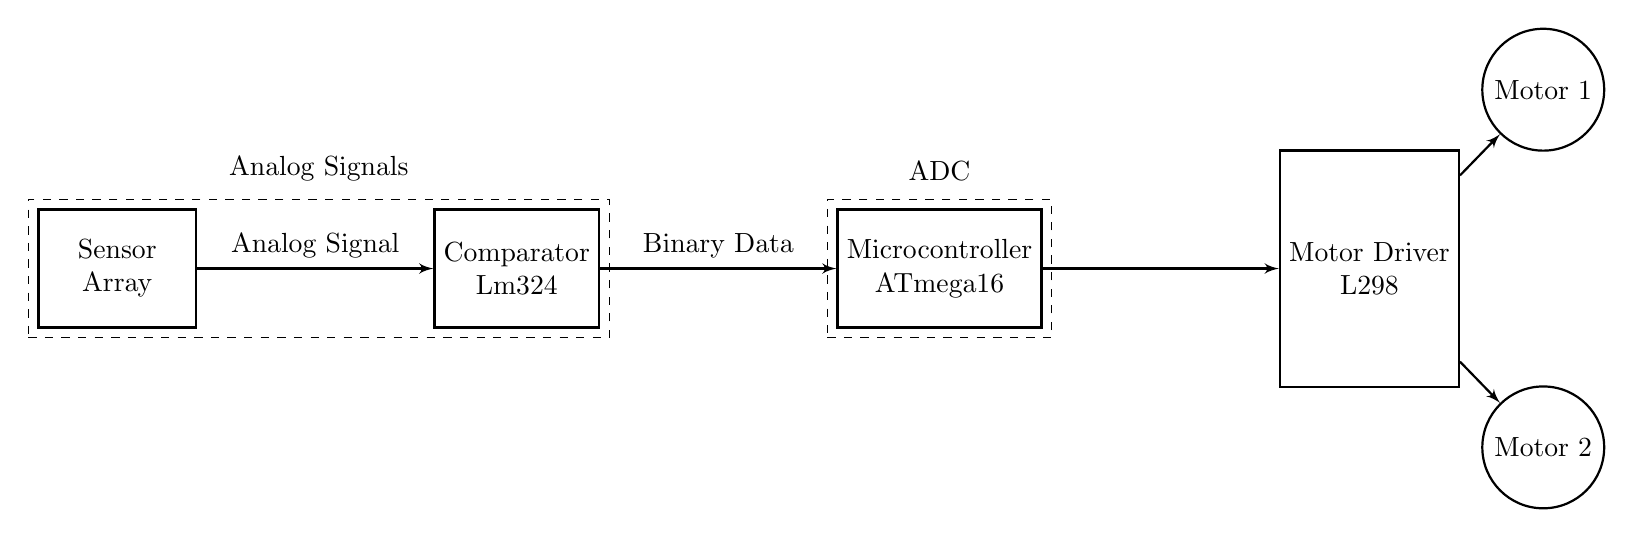
\begin{tikzpicture}[
    auto,
    block/.style={
        rectangle,
        draw,
        thick,
        minimum height=1.5cm,
        minimum width=2cm,
        align=center
    },
    motorblock/.style={
        rectangle,
        draw,
        thick,
        minimum height=3cm,
        minimum width=2cm,
        align=center
    },
    line/.style={draw, -latex', thick}
]

% Blocks with more horizontal spacing
\node [block] (sensor) {Sensor\\Array};

\node [block, right=3cm of sensor] (comparator) {Comparator\\Lm324};

\node [block, right=3cm of comparator] (micro) {Microcontroller\\ATmega16};

\node [motorblock, right=3cm of micro] (driver) {Motor Driver\\L298};

% Motors with adjusted positioning
\node [circle, draw, thick, minimum size=1cm, above right=0.2cm and 0.5cm of driver] (motor1) {Motor 1};
\node [circle, draw, thick, minimum size=1cm, below right=0.2cm and 0.5cm of driver] (motor2) {Motor 2};

% Connections with labels
\draw [line] (sensor) -- node[above] {Analog Signal} (comparator);
\draw [line] (comparator) -- node[above] {Binary Data} (micro);
\draw [line] (micro) -- (driver);
\draw [line] (driver) -- (motor1);
\draw [line] (driver) -- (motor2);

% Dashed boxes
\node [draw, dashed, fit={(sensor) (comparator)}] (analog) {};
\node [above=0.1cm of analog] {Analog Signals};

\node [draw, dashed, fit={(micro)}] (adc) {};
\node [above=0.1cm of adc] {ADC};

\end{tikzpicture}

\end{document}